\documentclass{report}

\usepackage{tikz}
\usetikzlibrary{positioning,shapes,shadows,arrows} 
 
 % Define block styles
 \tikzstyle{decision} = [diamond, draw, fill=blue!20, text width=4.5em, text badly centered, node distance=3cm, inner sep=0pt]
 \tikzstyle{data} = [draw, rectangle, fill=red!20, node distance=3cm, text centered, text width=6em, rounded corners, minimum height=3em]
 \tikzstyle{line} = [draw, -latex']
 \tikzstyle{computing} = [rectangle, draw, fill=blue!20, text width=5em, text centered, minimum height=4em] 

 \pgfdeclarelayer{background}
 \pgfdeclarelayer{foreground}
 \pgfsetlayers{background,main,foreground}
%----------------------

\title{Analysis and Design Document \\ for \\ OPAL}
\begin{document}
\maketitle
\chapter{Introduction}

\par The primary goal is create a framework that helps the users to realize the tunning task following the schema


\begin{figure}[htpb]
  \centering
  
  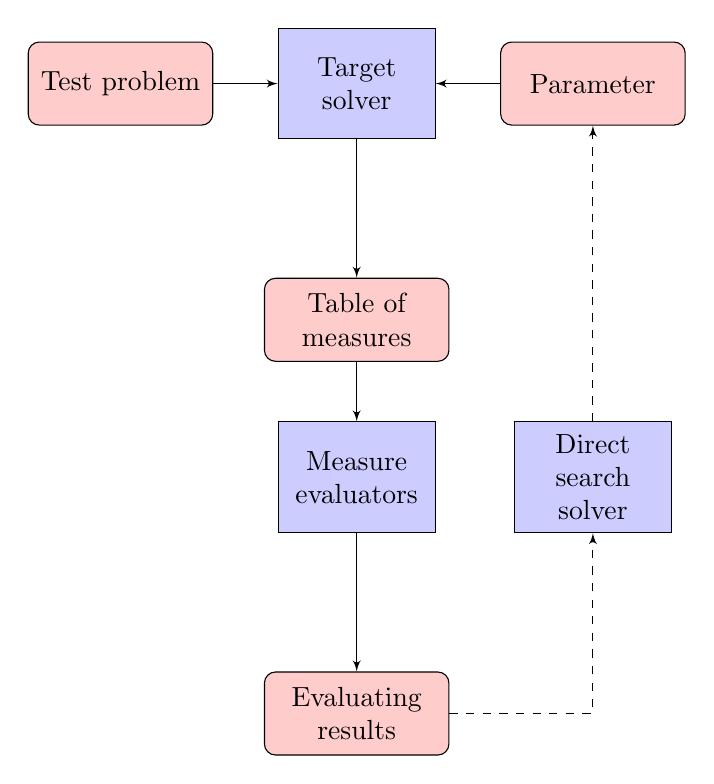
\begin{tikzpicture}[node distance = 2cm, auto]
    % Place nodes
    \node [computing] (algorithm) {Target solver};
    \node [data,left of=algorithm] (test-prob) {Test problem};
    \node [data, right of=algorithm] (param) {Parameter};
    \node [data, below of=algorithm] (measure-table) {Table of measures};
    \node [computing, below of=measure-table] (evaluator) {Measure evaluators};
    %\node [data, left of=evaluator, node distance=3.5cm] (model) {Evaluating model};
    \node [data, below of=evaluator] (evaluating-results) {Evaluating results};
    \node [computing, right of=evaluator, node distance=3cm] (solver) {Direct search solver};
    % Draw edges
    \path [line] (test-prob) -- (algorithm);
    \path [line] (param) -- (algorithm);
    \path [line] (algorithm) -- (measure-table);
    \path [line] (measure-table) -- (evaluator);
    %\path [line] (model) -- (evaluator);
    \path [line] (evaluator) -- (evaluating-results);
    \path [line,dashed] (evaluating-results) -| (solver);
    \path [line,dashed] (solver) -- (param);
\end{tikzpicture}
  \caption{General schema of parameter tunning}
  \label{fig:parameter-tunning-schema}
\end{figure}
\chapter{Backgrounds}
\par The principles are built basing on the three observations
\begin{itemize}
\item The Optimization of Algorithmic parameters framework can be analyzed as either a proccessing data system or black-box optimization problem solving. 
\item We can decompose any data proccessing to the elementary things by Data-Operator principle
\item Problem solving is can be decomposed by Data-Operator principle.
\end{itemize}

\section{Decomposition a system by Data-Operator principle}
\begin{itemize}
\item There are main entities Data and Operator
  \begin{enumerate}
  \item Data is in fact set of elements with the methods set and get value. The 
    set is organized in the different structure like a scalar, a vector or a matrix ...
  \item Operator represent for an operation, so it has  the input and the output.
    It may has also parameters to generalize its functionality.
  \end{enumerate}
\item A Data is characterized by Name, Type, Value and Storage (file or in memory, ...). Many data entity 
  can be grouped to create a Data Set.
\item An Operator is characterized by its Input and Output. Input and Output may be either the Data or an Operator with
  only constraint that their type are the same. 
  \begin{enumerate}
  \item Input and Ouput are Data, the Operator is called Evaluator. 
  \item Input and Output are Operators, the Operator is called Manipulator. 
  \end{enumerate}
\item We can combine many Operators in different ways to get a Process that are actually 
  an Operator.
  \begin{enumerate}
  \item A process of two sequenial Operators is a such combination that: Output of the first Opearator is input 
    of the second Operator
  \item Cooperation: Two Operators have the same Input.
  \end{enumerate}
\item The relations between two Operators are:
  \begin{enumerate}
  \item Dependence: A manipulator depends on the others if it used the others to proccess 
    the Data
  \item Independence.
  \item Inclusion A manipulator can be decomposed as combinations of the others
  \item Cooperation
  \end{enumerate}
\end{itemize}

\section{Analyse solving proccess by Data-Operator principle}
\par A solving process for an optimization problem is defined by the following diagram:
\begin{figure}[htpb]
  % We need layers to draw the block diagram
  \centering
  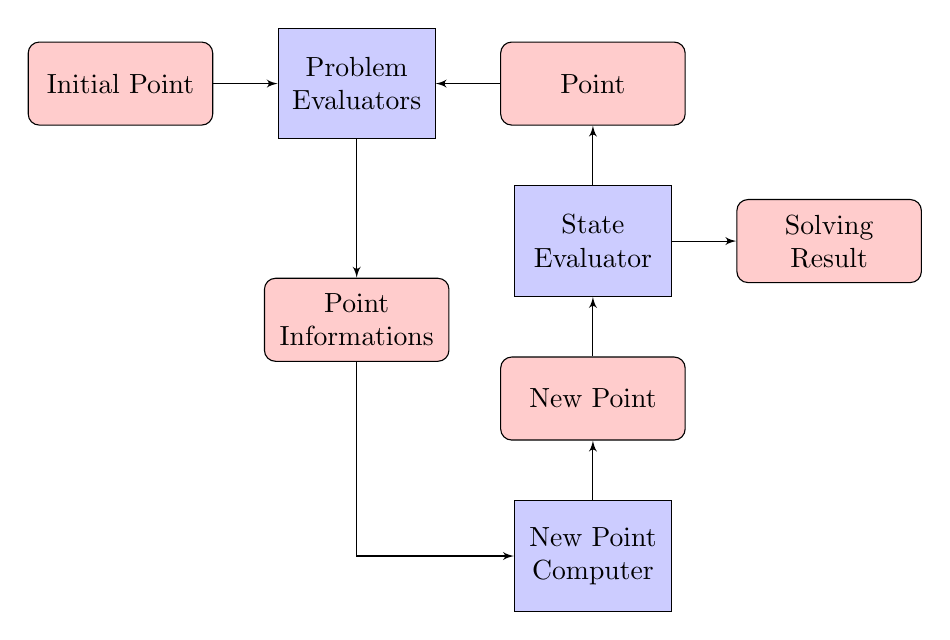
\begin{tikzpicture}[node distance = 2cm, auto]
    
    % Place nodes
    \node [computing] (evaluators) {Problem Evaluators};
    \node [data,left of=evaluators] (initial-point) {Initial Point};
    \node [data, below of=evaluators] (point-info) {Point Informations};
    \node [data, right of=evaluators] (point) {Point};
    \node [computing, below of=point, node distance = 2cm] (state-evaluator) {State Evaluator};
    \node [data, right of=state-evaluator] (opt-point) {Solving Result};
    \node [data, below of=state-evaluator,node distance=2cm] (new-point) {New Point};
    \node [computing, below of=new-point] (computer) {New Point Computer};
    
    % Draw edges
    \path [line] (initial-point) -- (evaluators);
    \path [line] (evaluators) -- (point-info);
    \path [line] (point-info) |- (computer);
    \path [line] (computer) -- (new-point);
    \path [line] (new-point) -- (state-evaluator);
    \path [line] (state-evaluator) -- (point);
    \path [line] (point) -- (evaluators);
    \path [line] (state-evaluator) -- (opt-point);
  \end{tikzpicture}
  \caption{Solving problem process}
  \label{fig:test-view}
\end{figure}

\chapter{System analysis}
We apply the principle above to describe the framework in a typical use-case. So, we try to analyse the framework in following steps:
\begin{enumerate}
\item Decompose the framework into the elementary thingss such that they are detail enough.
\item Identify and group the elements to describe the main components of our problem solving 
  proccesses as well the other supporting components.
\end{enumerate}

\section{Parameter Optimization is Data proccessing}
\begin{figure}[htpb]
  \centering
  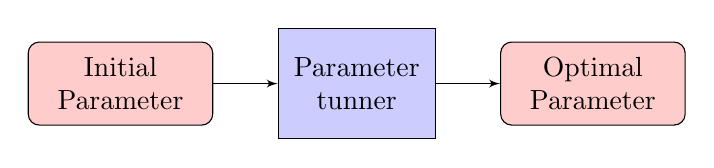
\begin{tikzpicture}[node distance = 2cm, auto]
    % Place nodes
    \node [computing] (tunner) {Parameter tunner};
    \node [data,left of=tunner] (initial-param) {Initial Parameter};
    \node [data, right of=tunner] (optimal-param) {Optimal Parameter};
    % Draw edges
    \path [line] (initial-param) -- (tunner);
    \path [line] (tunner) -- (optimal-param);
\end{tikzpicture}
  \caption{Top view of tunning parameter}
  \label{fig:top-view}
\end{figure}

\begin{figure}[htpb]
   % We need layers to draw the block diagram
  \centering
  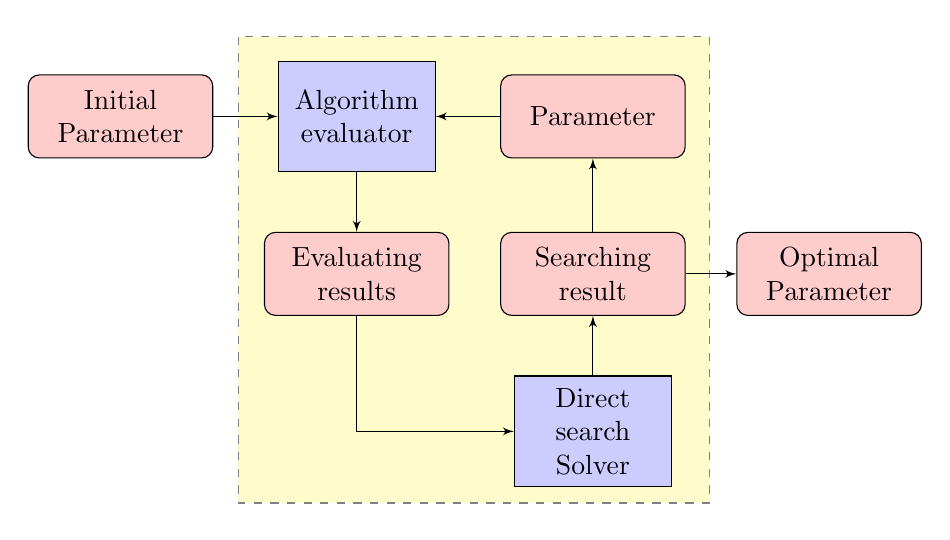
\begin{tikzpicture}[node distance = 2cm, auto]
   
    % Place nodes
    \node [computing] (evaluator) {Algorithm evaluator};
    \node [data,left of=evaluator] (initial-param) {Initial Parameter};
    \node [data, below of=evaluator, node distance = 2cm] (eval-result) {Evaluating results};
    \node [data, right of=evaluator] (param) { Parameter};
    \node [data, below of=param, node distance = 2cm](search-result) {Searching result};
    \node [data, right of=search-result] (optimal-param) {Optimal Parameter};
    \node [computing, below of=search-result] (solver) {Direct search Solver};
    % Draw edges
    \path [line] (initial-param) -- (evaluator);
    \path [line] (evaluator) -- (eval-result);
    \path [line] (eval-result) |- (solver);
    \path [line] (solver) -- (search-result);
    \path [line] (search-result) -- (param);
    \path [line] (param) -- (evaluator);
    \path [line] (search-result) -- (optimal-param);
    % Now it's time to draw the colored tunner rectangles.
    % To draw them behind the blocks we use pgf layers. This way we  
    % can use the above block coordinates to place the backgrounds   
    \begin{pgfonlayer}{background}
        % Compute a few helper coordinates
        \path (evaluator.west |- evaluator.north)+(-0.5,0.3) node (a) {};
        \path (solver.south -| param.east)+(+0.3,-0.2) node (b) {};
        \path[fill=yellow!20, draw=black!50, dashed]
            (a) rectangle (b);
    \end{pgfonlayer}
\end{tikzpicture}
  \caption{Black box optimization view of tunning parameter}
  \label{fig:blackbox-view}
\end{figure}

\begin{figure}[htpb]
   % We need layers to draw the block diagram
  \centering
  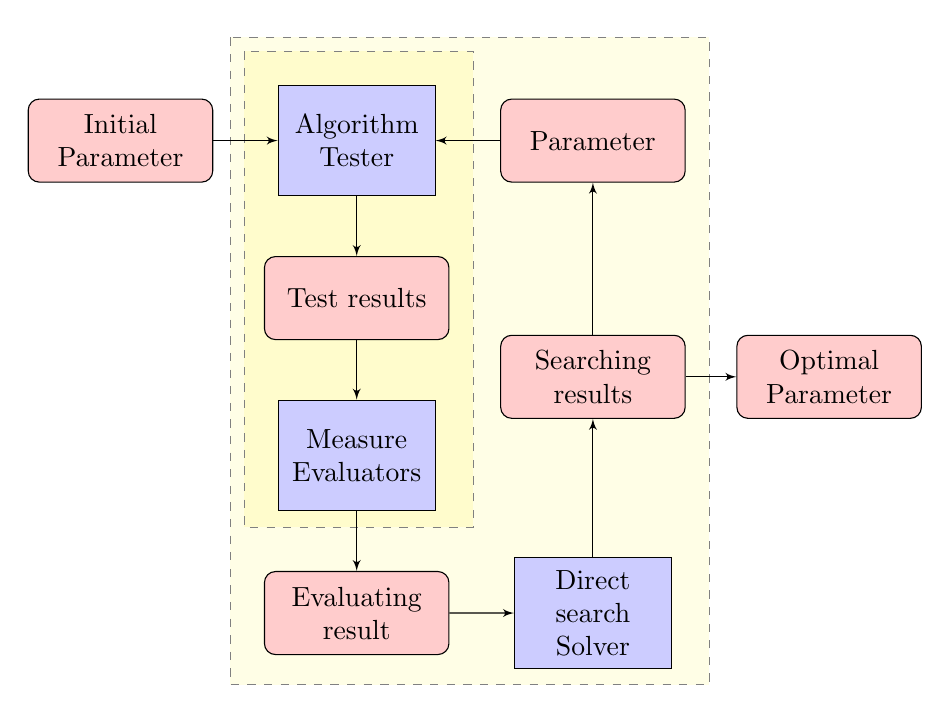
\begin{tikzpicture}[node distance = 2cm, auto]
   
    % Place nodes
    \node [computing] (algo-tester) {Algorithm Tester};
    \node [data,left of=algo-tester] (initial-param) {Initial Parameter};
    \node [data, below of=algo-tester,node distance = 2cm] (test-result) {Test results};
    \node [computing, below of=test-result] (evaluators) {Measure Evaluators};
    \node [data, below of=evaluators, node distance = 2cm] (eval-result) {Evaluating result};
    \node [data, right of=algo-tester] (param) { Parameter};
    \node [data, below of=param] (search-result) {Searching results};
    \node [data, right of=search-result] (optimal-param) {Optimal Parameter};
    \node [computing, below of=search-result, node distance = 3cm] (solver) {Direct search Solver};
    
    % Draw edges
    \path [line] (initial-param) -- (algo-tester);
    \path [line] (algo-tester) -- (test-result);
    \path [line] (test-result) -- (evaluators);
    \path [line] (evaluators) -- (eval-result);
    \path [line] (eval-result) -- (solver);
    \path [line] (solver) -- (search-result);
    \path [line] (search-result) -- (param);
    \path [line] (param) -- (algo-tester);
    \path [line] (search-result) -- (optimal-param);
    % Now it's time to draw the colored tunner rectangles.
    % To draw them behind the blocks we use pgf layers. This way we  
    % can use the above block coordinates to place the backgrounds   
    \begin{pgfonlayer}{background}
       % Compute a few helper coordinates
      \path (algo-tester.west |- algo-tester.north)+(-0.6,0.6) node (a) {};
      \path (solver.south -| param.east)+(+0.3,-0.2) node (b) {};
      \path[fill=yellow!10, draw=black!50, dashed]
      (a) rectangle (b);
      % Compute a few helper coordinates
      \path (a.west |- a.north)+(+0.3,-0.3) node (c) {};
      \path (evaluators.south -| test-result.east)+(+0.3,-0.2) node (b) {};
      \path[fill=yellow!20, draw=black!50, dashed]
      (c) rectangle (b);
     
    \end{pgfonlayer}
\end{tikzpicture}
  \caption{Empirical test view of tunning parameter}
  \label{fig:test-view}
\end{figure}

\begin{figure}[hpbt]
  \centering
  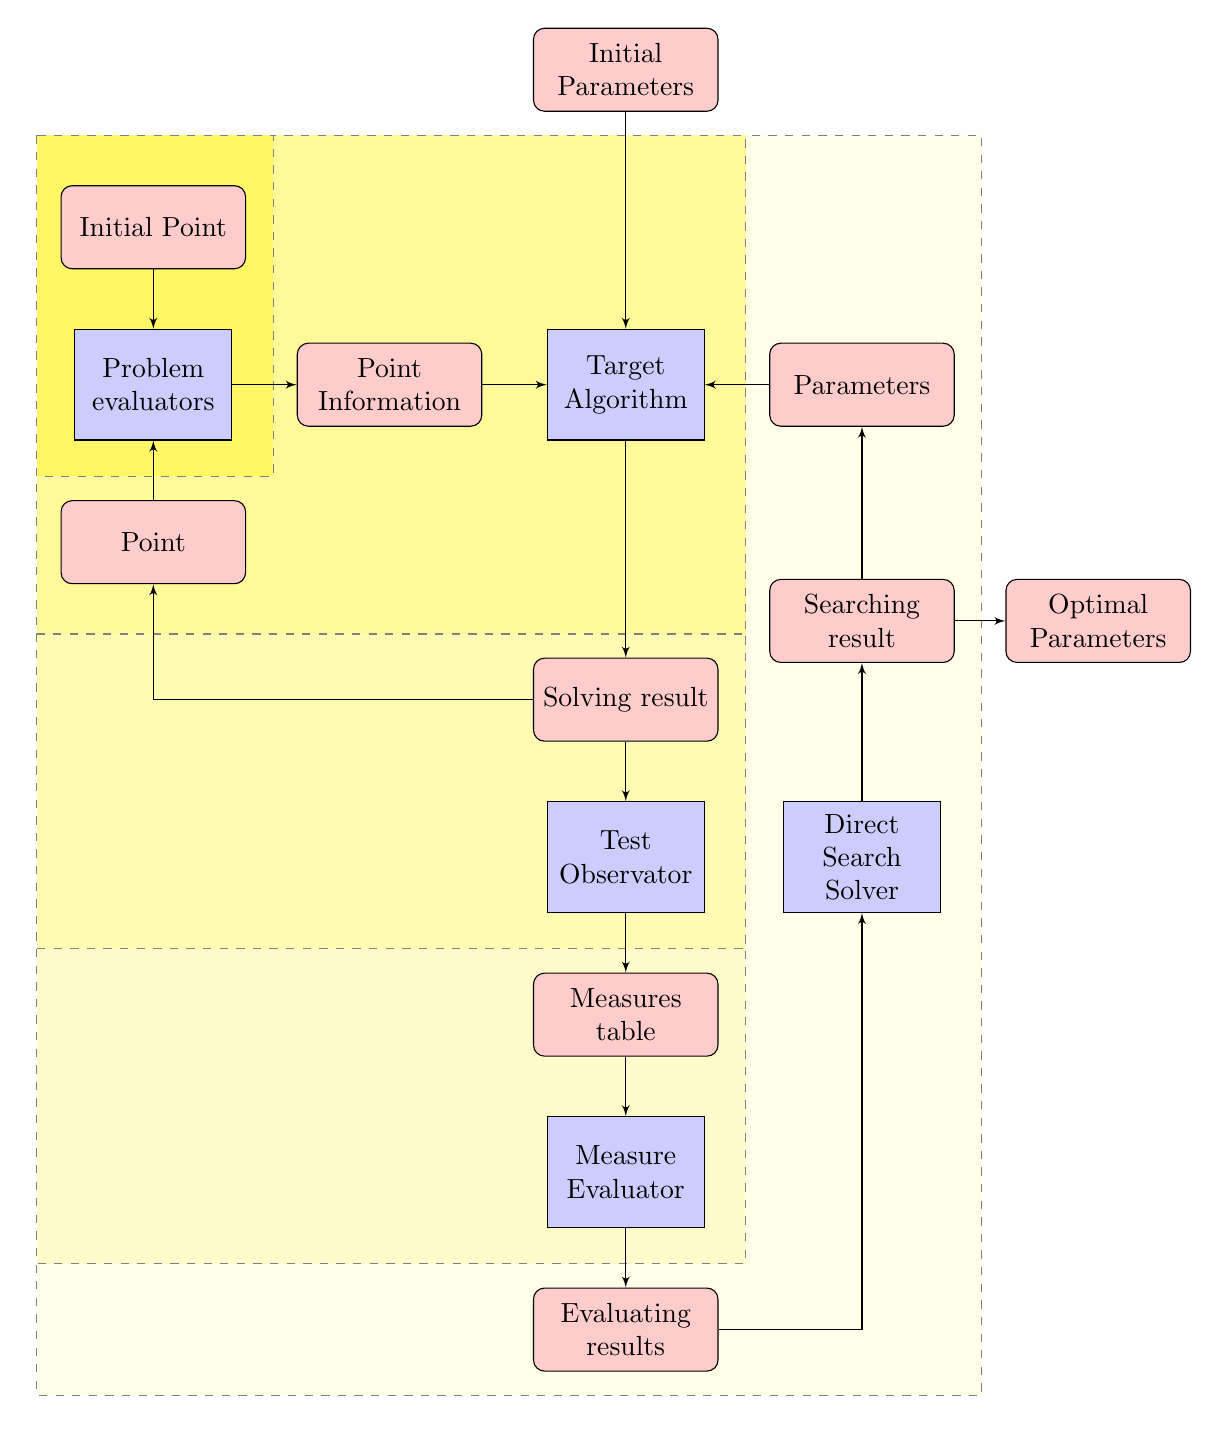
\begin{tikzpicture}[node distance=2cm, auto]
    \node [data] (initial-point){Initial Point};
    \node [computing, below of=initial-point](evaluator){Problem evaluators};
    \node [data, right of=evaluator, node distance=3cm](info){Point Information};
    \node [data, below of=evaluator, node distance=2cm](point){Point};
    \node [computing, right of=info, node distance=3cm](algorithm){Target Algorithm};
    \node [data, right of=algorithm](param){Parameters};
    \node [data, above of=algorithm, node distance= 4cm](initial-param){Initial Parameters};
    \node [data, below of=algorithm, node distance=4cm](solv-result){Solving result};
    \node [computing, below of=solv-result](test-observator){Test Observator};
    \node [data, below of=test-observator, node distance=2cm](measure-table){Measures table};
    \node [computing, below of=measure-table](measure-evaluators){Measure Evaluator};
    \node [data, below of=measure-evaluators, node distance=2cm](eval-result){Evaluating results};
    \node [data, below of=param](ds-solv-result){Searching result};
    \node [computing, below of=ds-solv-result,node distance=3cm](ds-solver){Direct Search Solver};
    \node [data, right of=ds-solv-result](opt-param){Optimal Parameters};

    \path [line](initial-point) -- (evaluator);
    \path [line](evaluator) -- (info);
    \path [line](info) -- (algorithm);
    \path [line](algorithm) -- (solv-result);
    \path [line](solv-result) -| (point);
    \path [line](point) -- (evaluator);
    \path [line](solv-result) -- (test-observator);
    \path [line](test-observator) -- (measure-table);
    \path [line](measure-table) -- (measure-evaluators); 
    \path [line](measure-evaluators) -- (eval-result);
    \path [line](eval-result) -| (ds-solver);
    \path [line](ds-solver) -- (ds-solv-result);
    \path [line](ds-solv-result) -- (param);
    \path [line](param) -- (algorithm);
    \path [line](initial-param) -- (algorithm);
    \path [line](ds-solv-result) -- (opt-param);
    \begin{pgfonlayer}{background}
       \path (initial-point.west |- initial-param.south)+(-0.3,-0.3) node (a) {};
       \path (opt-param.west |- eval-result.south)+(-0.3,-0.3) node (b) {};
       \path[fill=yellow!10, draw=black!50, dashed]
       (a) rectangle (b);
       
       \path (eval-result.north -| param.west)+(-0.3,0.3) node (b) {};
       \path[fill=yellow!20, draw=black!50, dashed]
       (a) rectangle (b);

       \path (measure-table.north -| param.west)+(-0.3,0.3) node (b) {};
       \path[fill=yellow!30, draw=black!50, dashed]
       (a) rectangle (b);
       
       \path (solv-result.north -| param.west)+(-0.3,0.3) node (b) {};
       \path[fill=yellow!40, draw=black!50, dashed]
       (a) rectangle (b);

       \path (point.north -| info.west)+(-0.3,0.3) node (b) {};
       \path[fill=yellow!60, draw=black!50, dashed]
       (a) rectangle (b);
    \end{pgfonlayer}
  \end{tikzpicture}
  \caption{Algorithm view}
  \label{fig:algorithm-view}
\end{figure}

\section{Parameter Optimization is Black Box Optimization problem solving}
\par There are two opimization problem solvings involed in parameter optimization.
\begin{itemize}
\item A Black box optimization problem is solved by a direct search solver
\item One or many test problems are solved by target solver 
\end{itemize}
\chapter{System design}
\par We try indentify three main types of objects in the above diagram: data, process and data manipulator
\begin{itemize}
\item Data that is the input, output and parameter of a process or a manipulator. Data has name, data type, 
  value and a propeties determine its physical storage that is either system standard output or a file. 
\item A manipulator represents for a data processing. It accepts a data object as input and return the other 
  data object that are the outputs. A manipulator may have one or many parameters that are the data objects 
  too to generalize the function. One thing important to define a manipulator is definition his function of 
  data processing.
\item A process is in general the cooperation of two or many manipulators. From the black box view, a process
  is a manipulator with input, output and parameters except that we don't need to specify its functionality.
\end{itemize}

\section{Process hiearachy}
\par By showing  the process hiearachy, we would like emphasize that, in our system, a process can be specified 
in two ways:
\begin{itemize}
\item Treat as a black box by specifying input, output and how to run.
\item Specify the sub-processes and the evaluators of the process and the their combinations. For our 
framework, the combinations are pre-defined, it is so enough to figure out the sub-process. In most of case, 
the users build up a process from a sub-process and an evaluator 
\end{itemize}
\tikzstyle{manipulator}=[rectangle, draw=black, rounded corners, fill=blue!40, drop shadow,
        text centered, anchor=north, text=black, text width=3cm]
\tikzstyle{process}=[rectangle, draw=black, rounded corners, fill=yellow!40, drop shadow,
        text centered, anchor=north, text=red!50, text width=3cm]
\tikzstyle{belongs}=[-o,draw]

\begin{figure}[hpbt]
  \centering
  \begin{tikzpicture}{node distance=2cm}
    \node (tunning) [process]
    {
      \textbf{OPAL Tunning}
    };
    \node (AuxNode01) [text width=1cm, below=of tunning, node distance=3cm] {};
    \node (evaluating) [process, below left=-0.5cm of AuxNode01]
    {
      \textbf{Algorithm evaluating} (Black box)
    };
    \node (ds-solver) [manipulator, below right=-0.5cm of AuxNode01]
    {
      \textbf{DS solver searching}
    };
    \path (tunning.west |- tunning.south) + (1.0, 0.1) node (a) {};
    \draw[belongs] (evaluating.north) -- (a);
    \path (tunning.south -| tunning.east) + (-1.0, 0.1) node (a) {};
    \draw[belongs] (ds-solver.north) -- (a);

    \node (AuxNode01) [text width=1cm, below=of evaluating, node distance=3cm] {};
    \node (testing) [process, below left=-0.5cm of AuxNode01]
    {
      \textbf{Algorithm testing} 
    };
    \node (measure-evaluators) [manipulator, below right=-0.5cm of AuxNode01]
    {
      \textbf{Measure Evaluators}
    };
    \path (evaluating.west |- evaluating.south) + (1.0, 0.1) node (a) {};
    \draw[belongs] (testing.north) -- (a);
    \path (evaluating.south -| evaluating.east) + (-1.0, 0.1) node (a) {};
    \draw[belongs] (measure-evaluators.north) -- (a);
    
    \node (AuxNode01) [text width=1cm, below=of testing, node distance=3cm] {};
    \node (solving) [process, below left=-0.5cm of AuxNode01]
    {
      \textbf{Problem solving} 
    };
    \node (observators) [manipulator, below right=-0.5cm of AuxNode01]
    {
      \textbf{Test observators}
    };
    \path (testing.west |- testing.south) + (1.0, 0.1) node (a) {};
    \draw[belongs] (solving.north) -- (a);
    \path (testing.south -| testing.east) + (-1.0, 0.1) node (a) {};
    \draw[belongs] (observators.north) -- (a);
    
    \node (AuxNode01) [text width=1cm, below=of solving, node distance=3cm] {};
    \node (defining) [process, below left=-0.5cm of AuxNode01]
    {
      \textbf{Problem defining} 
    };
    \node (solver) [manipulator, below right=-0.5cm of AuxNode01]
    {
      \textbf{Target solver searching}
    };
    \path (solving.west |- solving.south) + (1.0, 0.1) node (a) {};
    \draw[belongs] (defining.north) -- (a);
    \path (solving.south -| solving.east) + (-1.0, 0.1) node (a) {};
    \draw[belongs] (solver.north) -- (a);
  \end{tikzpicture}
  \caption{Manipulator hierachy}
  \label{fig:manipulator-hierachy}
\end{figure}
\section{Problem and solver}
\par The two elementary objects in a problem solving are built up from the Data, Evaluator and Operator.
\begin{itemize}
\item Problem includes a data set and one or many evaluator. For example, an optimization problem we need 
  an initial point and one or many evaluators representing for its model like objective 
  function computing, constraints computing, objective function gradient. Note the structure such as linearity, 
  is embeded as the structure 
\item Solver is specified with a searching process that created by combining the model computing process in 
  problem definition with an evaluator that compute new point from the information of current point (or model value).
  Search proccess is a loop process having the state, and the input is data (for example initial point) of 
  problem definition.
\end{itemize}

\end{document}